\documentclass{beamer}

\usepackage{graphicx}
\usepackage{subcaption}
\usepackage{ragged2e}
\usepackage[normalem]{ulem}
\usepackage[export]{adjustbox}
\usepackage{multicol}
\usepackage{hyperref}

\graphicspath{ {./images/} }

\hypersetup{
	colorlinks=true,
	linkcolor=blue,
	urlcolor=blue
}
\usetheme{Boadilla}

\title{How to become a generic gaming YouTuber}
\subtitle{Profitting off of children with minimal effort}
\author{Ondřej Staněk}
\institute{V.A}

\date{\today}

\begin{document}

\AtBeginSection[]{
	\begin{frame}
		\centering
		\begin{beamercolorbox}[center,shadow=true,rounded=true]{title}
			\usebeamerfont{title}\insertsectionhead\par
		\end{beamercolorbox}
	\end{frame}
}

\begin{frame}
	\titlepage
\end{frame}

\begin{frame}
	\frametitle{Glossary}

	\begin{description}
		\item[a channel] An account on YouTube that the author can post videos and other content to
		\item[slop] Low effort content, usually authored by artificial intelligence
		\item[an asset] Any component, model, process or framework of value that can be leveraged or reused (an
		      example of an asset is, for the purposes of this presentation, \textbf{an image})
		\item[metadata] Data that provides information about other data
	\end{description}
\end{frame}

\begin{frame}
	\frametitle{Table of contents}
	\tableofcontents
\end{frame}

\section{The first stage: Preparation}
\begin{frame}
	\frametitle{Picking a game}

	\begin{columns}
		\column{0.5\textwidth}
		
\includegraphics[width=5cm, center]{minecraft-logo.png}
		\column{0.5\textwidth}
		\centering
		
\includegraphics[width=5cm, center]{fortnite-logo.png}
	\end{columns}

	\begin{center}
		\href{https://www.twitch.tv/directory/gaming}{Twitch categories}
	\end{center}
\end{frame}

\begin{frame}
	\frametitle{Choosing hardware}

	\begin{columns}
		\column{0.5\textwidth}
		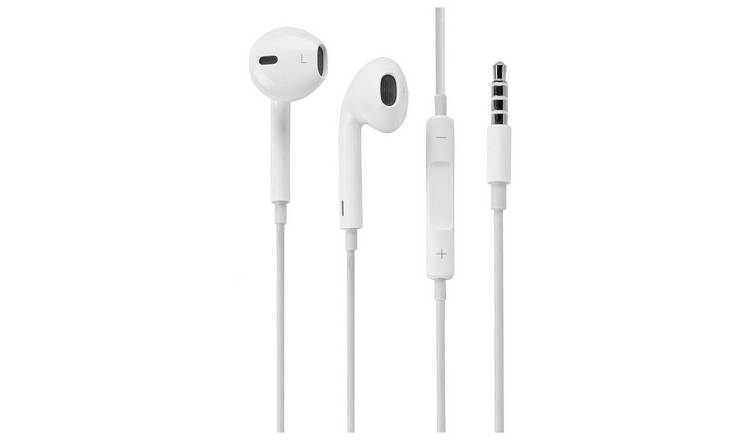
\includegraphics[width=5cm, center]{apple-earpods.jpg}
		\column{0.5\textwidth}
		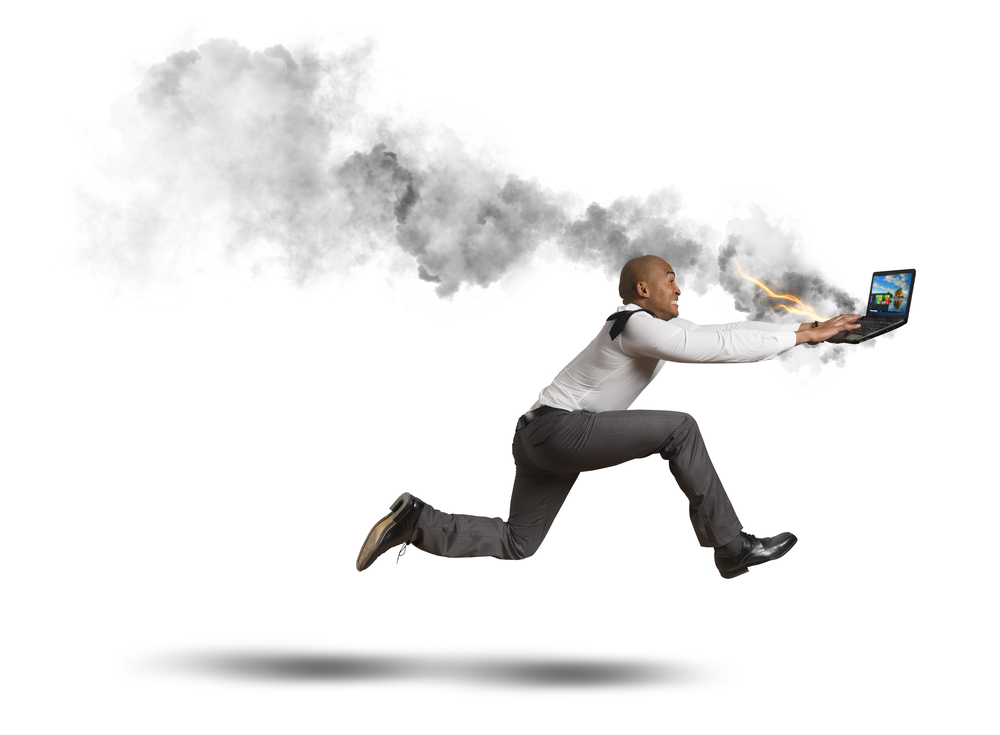
\includegraphics[width=5cm, center]{laptop-overheating.jpg}
	\end{columns}
\end{frame}

\begin{frame}
	\frametitle{Assets}
	\begin{columns}
		\column{0.5\textwidth}
		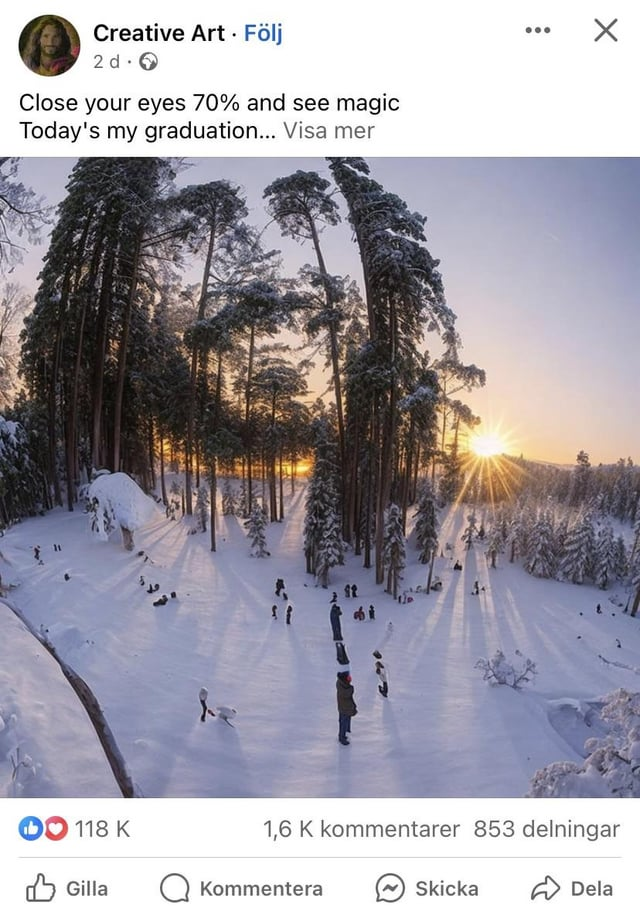
\includegraphics[width=5cm, center]{jesus-ai-slop.jpg}
		\column{0.5\textwidth}
		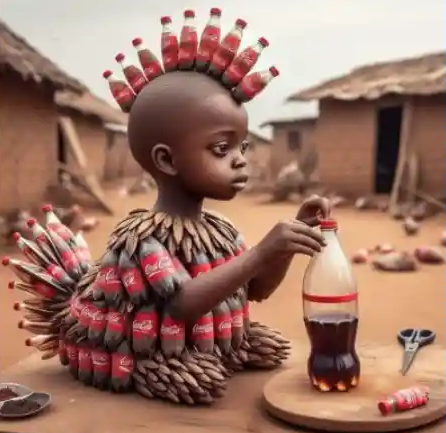
\includegraphics[width=5cm, center]{baby-with-chicken.png}
	\end{columns}

	\begin{center}
		\href{https://perchance.org/ai-text-to-image-generator}{Perchance AI image generator},
		\href{https://huggingface.co/chat}{HuggingChat}
	\end{center}
\end{frame}

\section{The second stage: Setting up your channel}
\begin{frame}
	\frametitle{Creating your Google account}

	\begin{columns}
		\column{0.3\textwidth}
		
\includegraphics[width=5cm,center]{google-account-setup/account-info.png}
		\column{0.3\textwidth}
		
\includegraphics[width=4cm,center]{google-account-setup/profile-picture.png}
		% prompt: youtube gaming profile picture with skibidi toilet g-man
	\end{columns}

	\vskip 0.6cm

	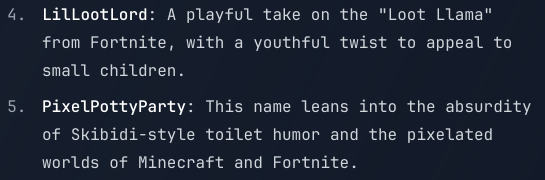
\includegraphics[width=6cm,center]{google-account-setup/usernames.png}
	% prompt: Generate a username for a YouTube channel that posts videos about Fortnite and
	% 	Minecraft, mainly targets small children and is infested with Skibidi toilet and the like
\end{frame}

\section{The third stage: producing \textit{"content"}}
\begin{frame}
	\frametitle{Videos}

	\begin{itemize}
		\item Your videos should have $>10$ minutes
		      \begin{itemize}
			      \item YouTube favours videos longer than 10 minutes
			      \item Your video will get mid-roll ads
			      \item More views means more ads, which means more money
		      \end{itemize}
		\item Titles and thumbnails should be \sout{clickbait} \textbf{exciting}
		      \begin{itemize}
			      \item Children are more likely to click/tap on a video with lots of colours,
			            explosions and exclamation marks in the metadata
		      \end{itemize}
		\item Videos should change topics/themes often \textit{enough}
		      \begin{itemize}
			      \item The average child has a short attention span
			      \item You need to make frequent cuts, insert funny sounds, pictures, music and other
			            content (like Family Guy clips) to entertain your target audience
		      \end{itemize}
	\end{itemize}
\end{frame}

\begin{frame}
	\frametitle{Editing}

	\begin{itemize}
		\item If you are lazy, you can use something simple like \href{https://shotcut.org}{Shotcut}
		      \begin{itemize}
			      \item Simple, easy to get started
			      \item Open source, completely
			            \href{https://www.gnu.org/philosophy/free-sw.html}{free} \textit{(libre)}
			      \item Licensed under the GPLv3
		      \end{itemize}
		\item For more complex editing, I recommend Black Magic Design's enterprise-grade
		      \href{https://www.blackmagicdesign.com/products/davinciresolve}{DaVinci Resolve}
		      \begin{itemize}
			      \item Closed source, proprietary
			      \item Requires a more powerful computer
			      \item Supports a more streamlined workflow, e.g. file and asset management is
			            integrated into the editor
		      \end{itemize}
	\end{itemize}
\end{frame}

\begin{frame}
	\frametitle{Using AI}

	\begin{itemize}
		\item You should use AI for everything you can
		      \begin{itemize}
			      \item You get better value for your time
			      \item As a consequence, your YouTube channel becomes more viable as a source of
			            passive income the bigger it grows
			      \item Some examples of using AI like this include:
			            \begin{enumerate}
				            \item \textbf{You don't have to speak, at all} - you can just replace your
				                  voice with an AI generated one
				            \item \textbf{You can use images specifically generated for your use
					                  case} - your AI of choice will give you slop made to fit your needs
				            \item \textbf{If you ever run out of ideas...} - A \textit{"new"}
				                  idea is always just a few keystrokes away
			            \end{enumerate}
		      \end{itemize}
	\end{itemize}
\end{frame}

\section{Afterword}
\begin{frame}
	\frametitle{Sources and attribution}

	\begin{itemize}
		\item\href{https://www.freepnglogos.com/pics/minecraft-logo}{FreePNGLogos} (game logos)
		\item\href{https://huggingface.co}{HuggingFace} (an open source AI model registry, with chat)
		\item\href{https://perchance.org/ai-text-to-image-generator}{Perchance} (a free AI image
		      generator)
		\item\href{https://overleaf.com/learn/latex}{Overleaf} (a \LaTeX \ editor, although I use my
		      own, Overleaf has great syntax documentation)
		\item\href{https://duckduckgo.com}{DuckDuckGo} (the search engine I use, also the source
		      of most definitions)
		\item\href{https://wordnik.com}{Wordnik} (an English dictionary, a source of
		      definitions)
		\item\href{https://dictionary.cambridge.org/}{Cambridge Dictonary} (another English
		      dictionary, also a source of definitions)
	\end{itemize}
\end{frame}

\begin{frame}
	\frametitle{Document source code}

	This presentation was written in \LaTeX. You can view the document's source code on GitHub at
	\url{https://github.com/stanekondrej/presentations/5A-how-to}

	\hskip

	How to become a generic gaming YouTuber \copyright \ 2024 by Ondřej Staněk is licensed under CC BY-NC-SA
	4.0. To view a copy of this license, visit
	\url{https://creativecommons.org/licenses/by-nc-sa/4.0}
\end{frame}

\end{document}
